% \documentclass{article}
\documentclass{book}

\let\cleardoublepage\clearpage

\usepackage[english]{babel}

% Set page size and margins
% Replace `letterpaper' with `a4paper' for UK/EU standard size
\usepackage[letterpaper,top=2cm,bottom=2cm,left=3cm,right=3cm,marginparwidth=1.75cm]{geometry}
\usepackage{graphicx}
\usepackage{xcolor}
\usepackage[colorlinks=true,linkcolor=blue,citecolor=red]{hyperref}
% \setlength{\parindent}{0pt}

% \usepackage{natbib}
\newenvironment{abstract}{}{}
\usepackage{abstract}

\hypersetup{
    colorlinks=true,
    linkcolor=[RGB]{255,34,255},
    citecolor=[RGB]{255,34,255},
}

\title{Research Automation Perspective Paper}
\author{Shiro Takagi}

\begin{document}
\sloppy
\maketitle
\tableofcontents

\begin{abstract}
    In this paper, I propose a perspective on the realization of machine learning algorithms that can conduct research autonomously. First, I look back at what kind of activities research, which is the subject of automation, involves. Next, I review existing research attempting to automate each component of these research activities. Based on these, I propose ideas for the realization of artificial researchers who can conduct research autonomously, and suggest a roadmap and action plan to achieve them.
\end{abstract}

\chapter{Introduction}

\section{Background}
Research has greatly supported the development of humanity so far. It has enabled agents to deepen their understanding of themselves and the world around them, and in doing so, acquire new capabilities. In this sense, research is an extremely important activity.

\section{Purpose of this perspective paper}

The purpose of this paper is to discuss the possibility of automating this activity of research, that is, the realization of intelligent agents capable of conducting research autonomously. After summarizing attempts at research automation so far, I intend to present my personal perspective on promising ideas, necessary elements, and ways to proceed in order to create artificial researchers. In particular, this paper is aimed at machine learning researchers and developers, with the goal of increasing the number of colleagues aiming for research automation by providing concrete possible actions.

One thing to note here is that my aim is not to automate or substitute the current research tasks, but to create intelligent agents capable of conducting research. In other words, as long as it is research, automated research may at first glance seem to be far removed from the current research activities. This is because the current research activity may not necessarily be the absolute optimal form in light of its purpose. 

First, the optimal form is always influenced by the context of history. Of course, the optimum in the era when letterpress printing was mainstream is different from the optimum in the era when the Internet became infrastructure. Research itself has changed its form over time, and the optimal form of research in the present or future can naturally change. Moreover, as Nielsen and Qiu say \cite{nielsen}, it is believed that we have only explored a very limited range regarding the practice of research. The establishment of current research practices is a very recent event in human history, and we may not yet have arrived at the optimum way of intellectual production. Furthermore, current research assumes that humans are the main creators of knowledge. This naturally imposes human cognitive constraints, which may significantly limit the range of activities that can be conducted for knowledge production. 

Therefore, instead of thinking about how to automate and streamline current tasks, I discuss the possibility of realizing intelligent agents that can autonomously perform the fundamental and core elements of research activity in a more optimal form, and what is necessary for this.

\section{Continual update of this paper}

Additionally, this paper is intended to be updated on an ongoing basis. If you find points that you think are lacking or inaccuracies in understanding, please send a Pull Request on GitHub. Based on that, I will revise the content of the paper as needed.


\chapter{What is Research?}

To create an agent capable of conducting research autonomously, it is crucial to understand what research is in the first place. Therefore, in this chapter, I would like to discuss the characteristics of what is called research.

However, my aim here is not to identify a universal, historically independent, and absolutely singular definition of what research is. It seems almost impossible to specify such a thing \cite{chalmers2013thing,sep-scientific-method}. I do not totally believe that I, a layperson in the philosophy of science, could provide an answer to a question that has yet to be resolved even within the philosophy of science.

Rather, my goal is to endeavor to describe various characteristics of research to the extent that it can provide a starting point for engineers and information scientists who aim for autonomous research capabilities. To that end, I first discuss a possible working definition of research.

\section{A Working Definition of Research}

\subsection{Research as Knowledge Production}
One commonly mentioned definition of research is the act of generating new knowledge. For instance, research of mathematics create unknown proofs of theorems, physics elucidates unknown natural laws, and engineering produces blueprints for never existed things. I will adopt this definition as the working definition in this paper. \textbf{Therefore, whenever I refer to research in the following, please interpret it as discussing the knowledge production.} \textcolor{red}{TODO: add examples}

The reason why I deliberately use the word research instead of science is because I want to include fields like humanities and arts, which are not typically referred to as science, within the scope of automation in the long run. Science refers to a methodology for generating knowledge, and I believe that new knowledge is not necessarily produced only by scientific methods. I believe that so-called humanities and arts also share the commonality of producing new knowledge. Therefore, the definition of generating new knowledge can be said to encompass these fields as well.

Science is an extremely precise and robust  framework for knowledge production. Because of its power and popularity, most of the existing analysis on research is about science. Therefore, although this paper uses the word research, the automation of science will be at the center of our discussion. I plan to explore the analysis towards the automation of research in humanities and arts in future.

\subsection{Research as Belief Revision}
Before delving into how humans have been producing knowledge, let's think a bit deeper about what it means to produce knowledge. Defining knowledge rigorously is a philosophical debate that has not yet been settled, and I won't delve into it deeply here. 

Knowledge is what we know about a target. Thus, producing knowledge can be rephrased as the process of transitioning from a state of not knowing to a state of knowing about a certain target, i.e., transforming the unknown into the known. Research could possibly be perceived as a function that takes the unknown as input and outputs the known.

However, there's a problem here, as the binary approach of categorizing things into known and unknown often does not always hold true. In deductive disciplines such as mathematics and logic, this might be different, but in the case of empirical sciences, due to their inductive nature, we cannot strictly assert that a certain hypothesis is correct. For example, even if a theory has withstood tens of thousands of tests, it is fundamentally impossible to deny the possibility that it may fail on the next attempt. As Karl Popper once aptly put it, all we can do is strengthen our confidence in the hypothesis by continuing to subject it to falsification tests \cite{popper1959logic}.

When a hypothesis survives a test, it was said that our belief in the likelihood of the hypothesis strengthens. Empirical science implicitly assumes a principle that relies on inductive reasoning as the basis for these tests. For example, we believe that if the number of observations consistent with a certain claim increases, that claim is more likely to be valid (this is called the principle of confirmation). Additionally, we hold the belief that unless other factors change, what has held true so far will continue to hold true (this is called the principle of uniformity of nature). These principles of confirmation and uniformity are the foundations of inductive reasoning, and they are unavoidable in empirical science. However, both the principle of confirmation and the principle of uniformity are merely beliefs, and there is no guarantee anywhere that these are ``correct''. The reason these can serve as the foundation for testing is because these beliefs are far more solid than the belief in the likelihood of a hypothesis that someone has just recently presented. That is, empirical science could be described as an endeavor to update the likelihood of a hypothesis by tying the belief held about a certain hypothesis to a more solid belief. While mathematics and logic are rare examples, considering that all other research endeavors are fundamentally empirical, \textbf{it may be possible to rephrase the endeavor of research, that is, the production of knowledge, as largely an endeavor to update our belief in the correctness of a certain object.}

This position may have some similarities with a famous stance in philosophy of science that argues everything is, at its core, subjective, relative or a matter of belief \cite{chalmers2013thing,kerlinger1973structure,howson2006scientific}. However, what I want to emphasize here is that I think the characteristic of research lies in tying beliefs about an object to stronger beliefs. And I believe that it is this strength of conviction, which seems self-evident to many people, that lends objectivity and persuasiveness to the claims of science.

\subsection{Disclaimer Regarding the Characteristics of Research}
I have mentioned that research is an endeavor to transform the unknown into the known, but you may question what distinguishes it from other activities that appear to do the same. This issue arises from the fact that I have not properly defined knowledge in this paper. In this paper, I won't discuss this in detail but will limit myself to a brief disclaimer.

\subsubsection{Rigor of Methodology}
Firstly, you may wonder if anything unknown would suffice. I believe that research does not choose its subject and anything unknown is acceptable. Rather, what's important is the strictness of the methodology – whether the unknown truly became closer to the known, whether it was concluded into a stronger belief. Generally, the method employed by what we call research is designed with extreme precision, and as a result, it seems to withstand rigorous evaluations. This can be considered a major feature that distinguishes research from other various activities.

\subsubsection{Objectivity of Research}
Next, you might question whose known and whose belief we are talking about. Knowing or understanding something is a subjective experience. Therefore, you might wonder if it can be called research if what is unknown to person A becomes closer to the known for person A. At least the knowledge currently being produced by research does not seem to be of this kind. This is because the knowledge produced by research implicitly assumes it to be knowledge for humanity. In other words, what current research is doing is bringing what is unknown to humanity closer to the known. Therefore, the knowledge produced must be interpretable by other humans, and it is important that the results and procedures are objective, that is, they align with the stronger beliefs of more people.

The reason I deliberately distinguished between mere knowledge and knowledge for humanity is because I believe that there could be knowledge for beings other than humans. As I have repeated, understanding is subjective, so if machines start conducting research in the future, it is natural to think that there will be unknowns for machines and beliefs for machines. Therefore, it's possible that we could live in a world where humans produce knowledge for humans, machines produce knowledge for machines, we could live in a world where knowledge is produced for all agents including machines and humans, or we could continue living in a world where knowledge is produced solely for humans. In this sense, I believe one of the problems that will be questioned in the future is whose objectivity and whose belief we are talking about. I will discuss this point in more detail later.

\subsection{The Previous Discussions Regarding the Definition of Research (Scientific Discovery).}


In the previous section, I introduced my definition of research. Here, I will look back on the discussions that have taken place so far regarding the definition of research or scientific discoveries. Then, I will explain the correspondence between those discussions and the definition mentioned in the previous section. \textcolor{red}{TODO}

\section{Research Process}

% It is believed that research began with individual and concrete tasks. Among them, common actions were patterned and crystallized as a scientific method. We currently recognize this abstract set of behaviors as research. For example, hypothetico-deductive method and hypothesis testing are abstracted scientific method.

% Also, researchers use a research paper as a medium of knowledge transfer. Therefore, there are patterned activities related to a research paper. Examples of these include conducting surveys, gathering information from papers, and writing a thesis.

% Note that these are necessary tasks just because we use a paper as a medium of knowledge transfer, but they may not necessarily be indispensable for generating new knowledge. There are other such tasks as well. For example, peer review and fund raising are essential to current research practices in society, but they may not necessarily be indispensable for knowledge production.

% In this way, various tasks arise in conjunction with research. When considering the automation and optimization of research, it is desirable to consider streamlining all of these tasks. However, in this article, we focus on the process from determining a research topic to publishing a research paper. We will refer to this process simply as the \textit{research process} from here on.

% \subsection{Overview}

% As mentioned earlier, research is an attempt to turn the unknown into the known. Therefore, the research process can be seen as a function that takes the unknown as input and outputs the known. However, in reality, a single research paper may not be enough to turn the unknown into the known. Therefore, in practice, the research process is considered to be a procedure that takes the unknown as input, and outputs a text that describes the procedures and their results, as well as their interpretation, in order to turn the unknown into the known.

% First, let me structure the common research process. In particular, I will base the structuring of the research process on the method of empirical science, which many researches rely on as a foundation. However, I believe that this framework can be applied to other research activities, such as mathematics, as well. I will explain the reason for this later.

% The research process, especially that of empirical science, is carried out through the following steps: topic decision, hypothesis generation, verification design, verification, and analysis of experimental results. The outputs of these steps are then written into a paper, which undergoes peer review and is eventually published.

% Note that some commonly seen items, such as surveys, are not included here for a reason. First, as mentioned earlier, gathering information from papers is only a means of knowledge transfer through the use of a thesis. Second, information extraction from papers can be done at any stage of the research process. Thus, I believe that processing related to a paper, such as \textit{reading papers} and \textit{writing a paper}, needs to be considered separately from the aforementioned research process.

Next, I will discuss how human beings have been conducting research. I'll structurize the abstract pattern of the process (which I will call\textit{ research process}) from determining the unknown to it becoming known. I will pay a particular attention to the scientific methods established by empirical sciences. However, as will be mentioned later, I believe this pattern may implicitly apply to other research fields, such as mathematics and humanities as well. Also, I will try to distinguish and discuss these research processes into necessary components for knowledge production and those that are not. As previously mentioned, because humans are currently the primary creators of knowledge, there are many constraints that come from human society. When considering the possibility of machines conducting research in the future, it will be extremely important to distinguish and organize what is dependent on humans and what is not.

I believe that the conduct of human research can be roughly divided into three stages: knowledge production, knowledge evaluation, and knowledge sharing. Although these may not necessarily be distinctly separable from each other, I adopt this classification because it is useful for advancing discussion. The process of knowledge production consists largely of the steps: problem determination, hypothesis generation, verification design, and verification. And in this process, the ability to read and write documents and analyze data are required as necessary skills. Below, I will examine each of these in more detail. These are summarized in the Fig. \ref{fig:research_process}.

\begin{figure}[htb]
    \centering
    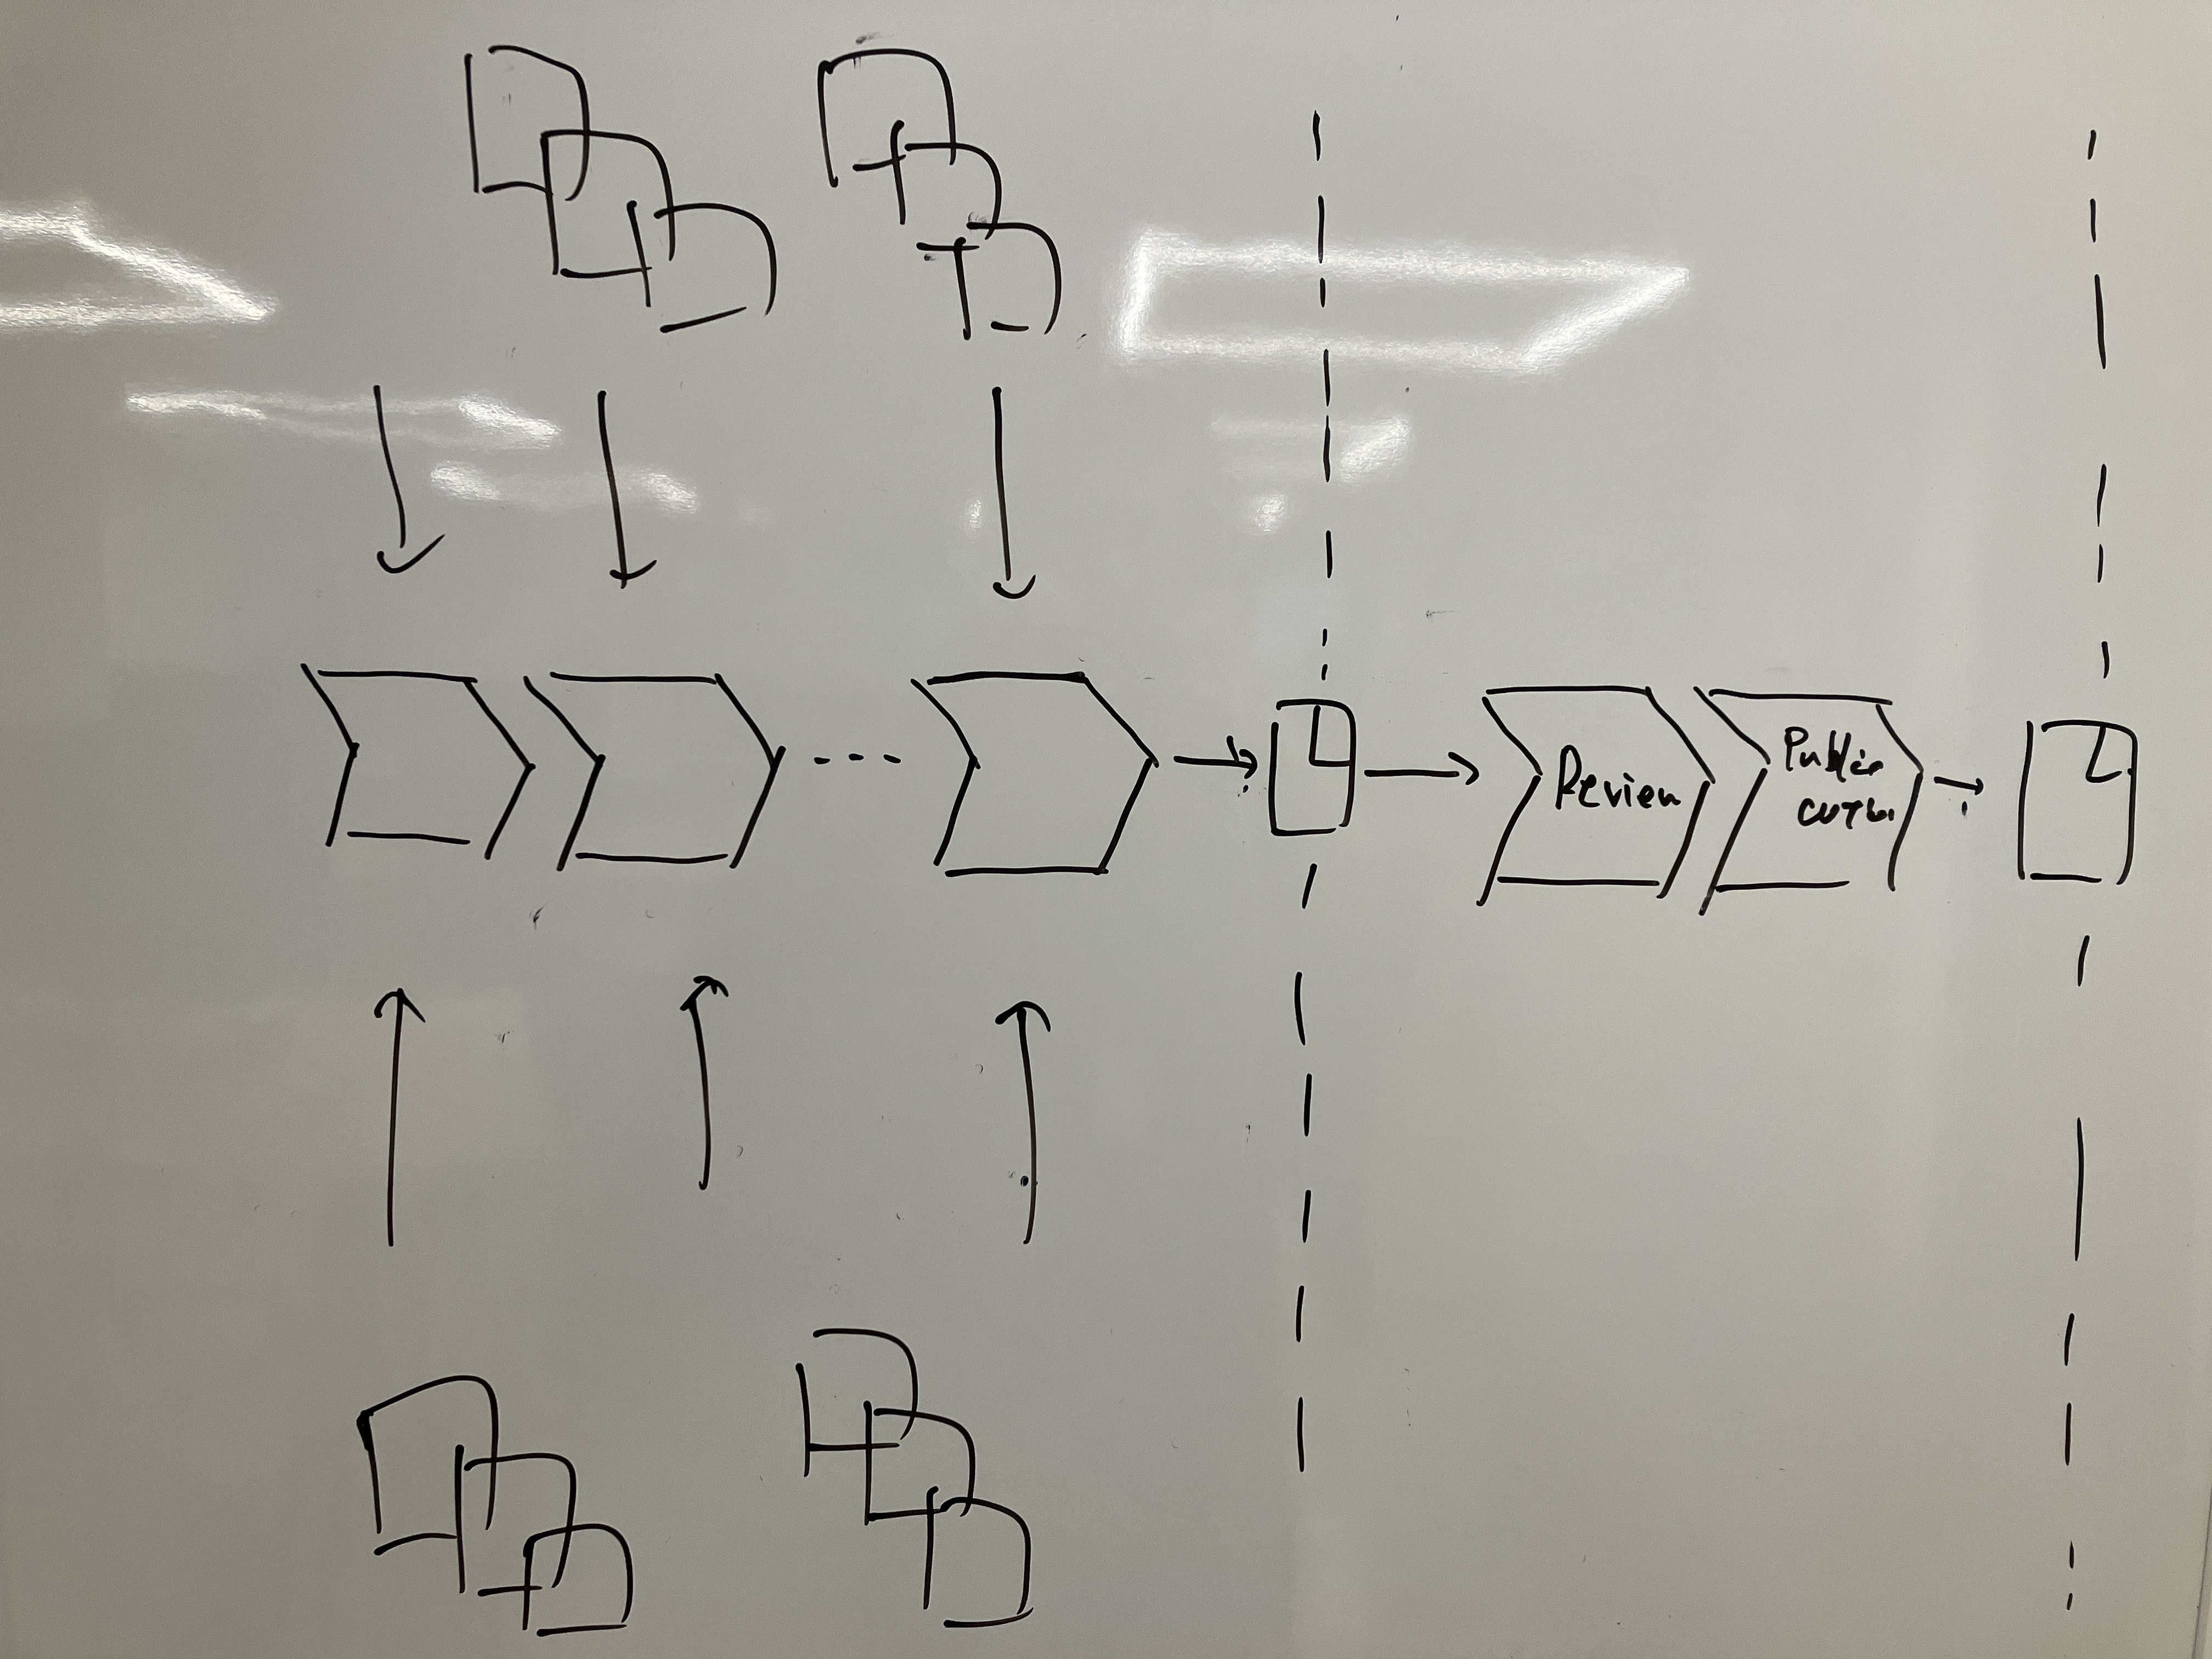
\includegraphics[width=\textwidth]{figs/researchprocess.jpg}
    \caption{Caption}
    \label{fig:research_process}
\end{figure}


This structuring is tentative and there may be a better way to structure the research process. However, I have created this structure for practical purposes in order to move the discussion forward. I hope the structure of this article be a starting point for conceiving a better structurization. I believe that structuring and deepening understanding of the elements that are essentially important for knowledge production is extremely crucial when aiming for the automation of research.

\subsection{Knowledge Production: Question Construction}
To transform the unknown into the known, we first need to determine the unknown that will be the subject, in other words, we must construct a research question. We approach the unknown to the known by asking questions, providing tentative answers to them, and then verifying the validity of those answers. 

Indeed, the idea that thinking of good questions is extremely important for research is widely accepted in the research community \cite{alon2009choose}. In other words, this means that we distinguish between questions that are important and those that are not, based on certain criteria. For example, \cite{alon2009choose} suggests that a good question is one that solves challenges facing the research community. We consider a question to be important if it generates knowledge that greatly contributes to a certain purpose. Valuing the degree of contribution to a purpose also implies viewing research as a form of problem-solving.

In practice, we seem to determine the questions we should tackle in this way, implicitly and explicitly. For example, let's say that someone try to answer a question of ``How neural networks have reasoning capability?'' in his/her study. This question may come from a thought process of ``I want to create artificial general intelligence, which requires systematic thinking, that needs ...'' In this case, the final purpose is to achieve ``artificial general intelligence'', and the question addressed as a result is ``ow neural networks have reasoning capability?'' In other words, when we want to conduct important research, we follow a process that starts with the goal we want to achieve, considers the tree of important unknowns that should be clarified for its achievement, and sets the end of that tree as the research question. This process is summarized in Fig. \ref{fig:unknown_tree}.

\begin{figure}[htb]
    \centering
    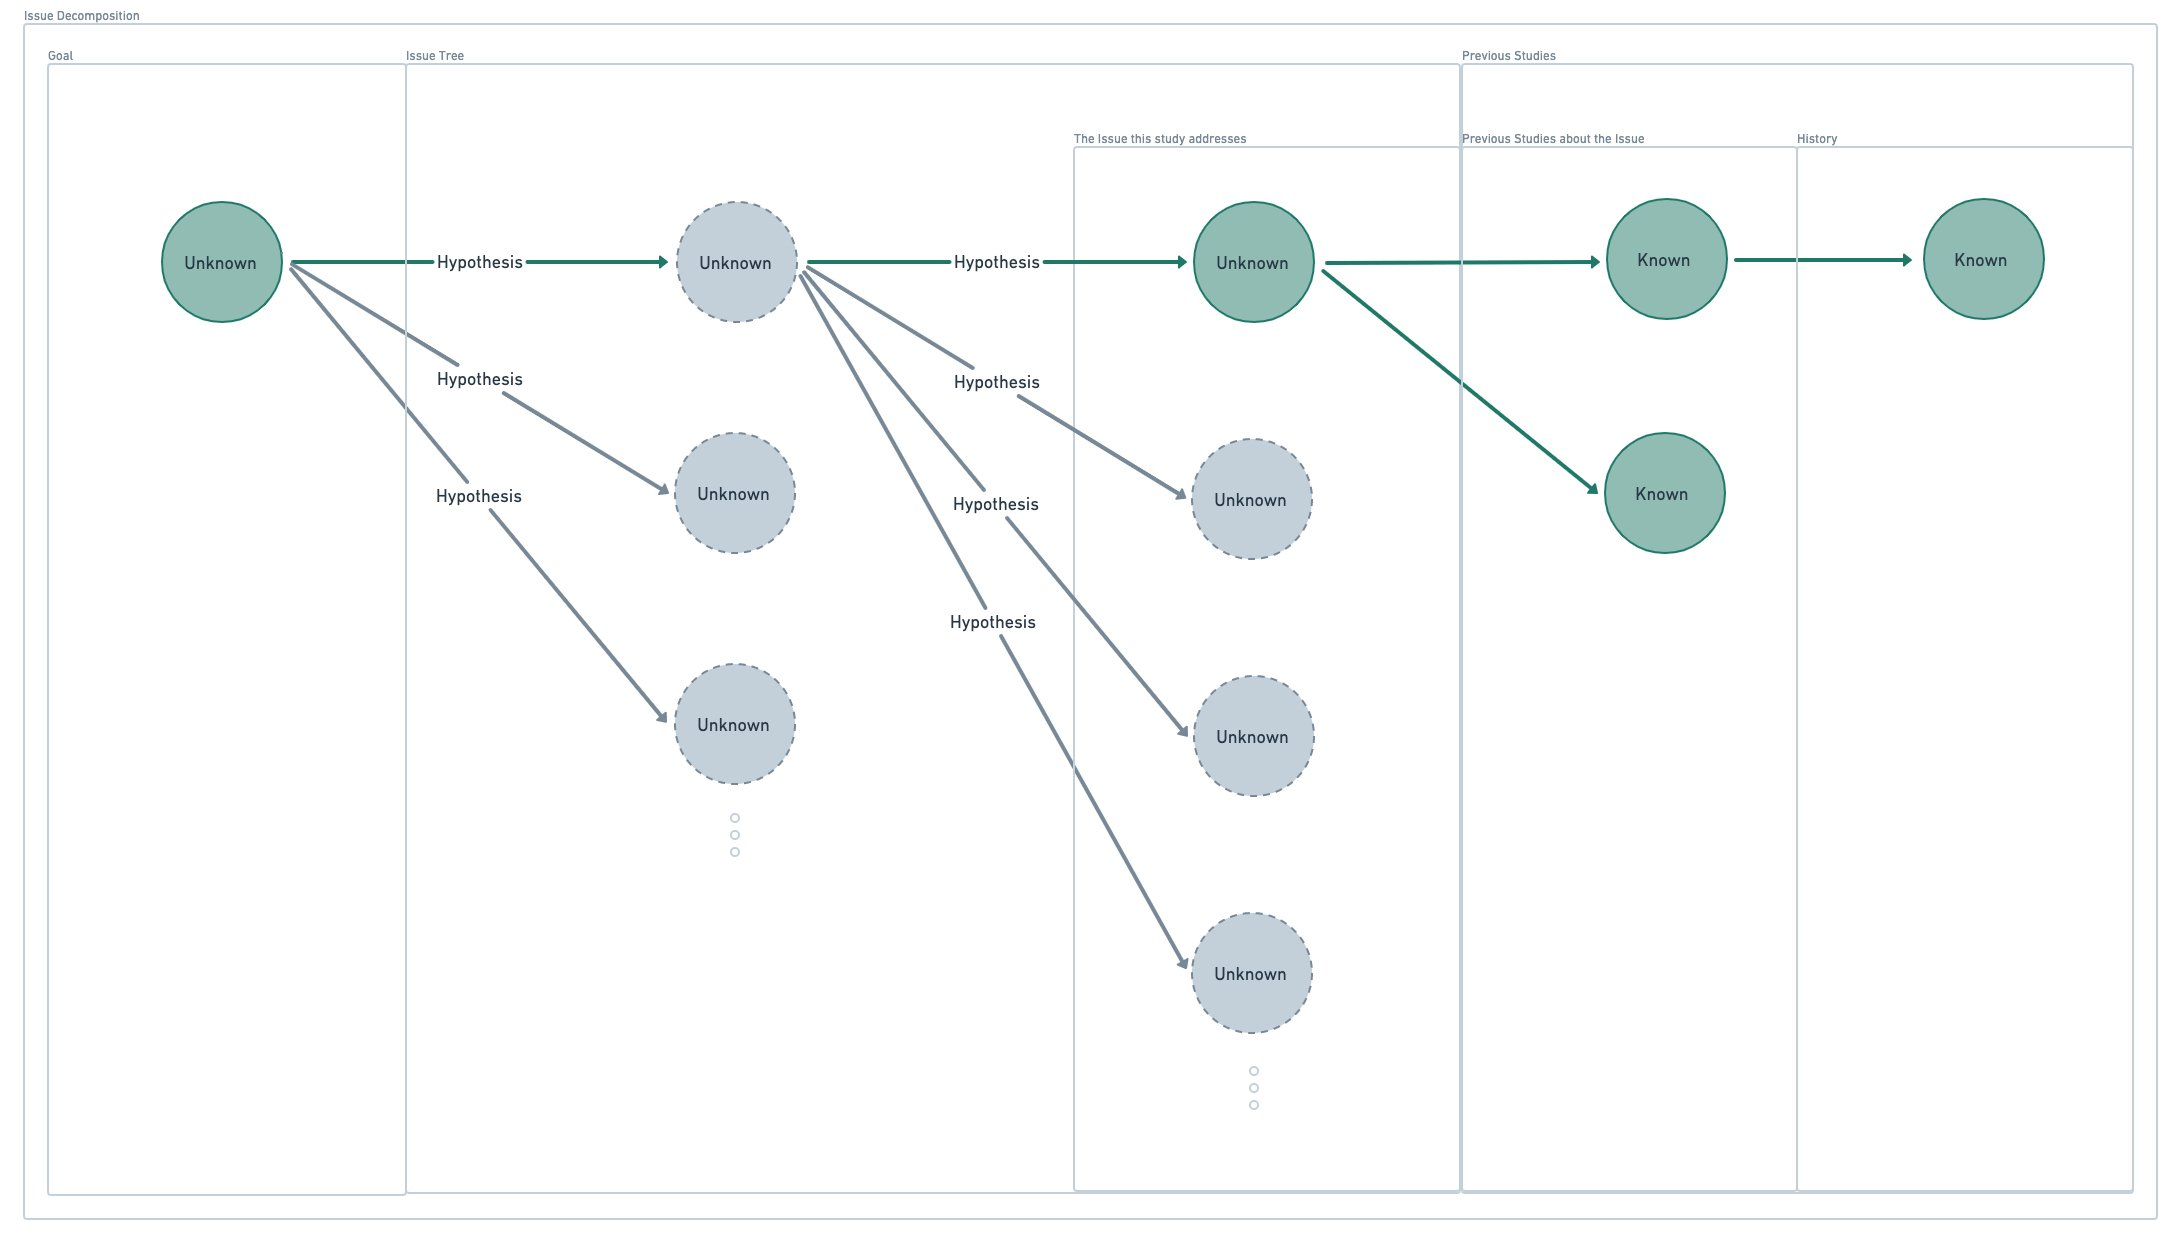
\includegraphics[width=\textwidth]{figs/unknown_tree.jpeg}
    \caption{Caption}
    \label{fig:unknown_tree}
\end{figure}

Of course, the purpose mentioned here may be a sub-goal of a higher-level goal. For example, the goal of ``creating general artificial intelligence'' may be a sub-goal of a more fundamental goal of ``satisfying intellectual curiosity,'' and the goal of ``satisfying intellectual curiosity'' may be biologically demanded for better exploration of the environment. These can lead to an infinite regression when considered strictly, so I won't delve into it any further here, but it could become an important issue when considering how to realize fully autonomous agent to construct questions.

Given these points, in realizing an agent that autonomously constructs questions, it may become important to consider how to automatically determine ``important questions,'' and how to acquire the ability to find goal-driven questions to solve for achieving the purpose. To achieve this, it would be important to first understand in more detail what kind of questions we consider important. It seems that we still lack an understanding of what kind of research questions are important, but in the field called \textit{science of science} \cite{wang2021}, which studies the research itself, scientific studies on research impact are also advancing. The insights gained here may provide important knowledge in building new algorithms and optimization metrics.

\subsubsection{Value-Neutral Question Construction}

So far, I have explained the importance of constructing good questions. However, in light of the definition of knowledge production, this is not necessarily required for knowledge production to be as it is. From the perspective of knowledge production, as long as the unknown is truly unknown and can be rigorously approached towards becoming known, there should be no problem. The unknown can be anything arbitrary, and knowledge production itself does not demand a specific nature for it. The importance or value of knowledge is inherently dependent on context, so the significance of a certain knowledge is not determined a priori from the moment it is generated. Importance becomes an issue only when that knowledge is intended to be generated within human society, implicitly assuming that humans will use it in some form. In other words, the demand for importance is a constraint imposed by human society not by knowledge production.

Science based on the importance of questions discussed above is a \textit{value-driven science} \cite{kitano2021nobel}. However, as previously mentioned, these may be due to cognitive constraints imposed by human society, including the inability to handle knowledge that is deemed ``unimportant.'' Therefore, when automating question generation, it may be possible to explore a wide range of questions, including those that were previously considered ``unimportant.'' In doing so, it is possible that knowledge that was not considered ``important'' according to previous criteria could actually be extremely significant. This is referred to as \textit{exploration-driven science} \cite{kitano2021nobel}, and it could become a new form of research liberated from constraints imposed by humans. 

Indeed, it is impossible to create a completely value-neutral system. All agent systems must have some form of bias. However, what I would like to emphasize is the potential to incorporate biases different from the criteria previously used by humans, and how this can enable us to consider more diverse approaches to research. This highlights the importance of creating agents capable of autonomously conducting research.

\subsubsection{Unknowness}
In the previous statement, it was mentioned that as long as the unknown is truly unknown and it can be approached towards becoming known, there should be no problem. The process of approaching the known will be explained in the next section, and here I will delve a bit more into the determination of unknownness. 

Currently, researchers often demonstrate the unknownness of a topic by referencing several previous studies in their papers and explaining that none of them have yet resolved the unknown. This implies the use of subjective evaluation criteria, where researchers examine several papers considered ``major literature'' in a field and consider them as unknown if none of them have provided an answer. Furthermore, as mentioned later, we evaluate the quality of research outcomes by having them assessed by a small number of experts in the same field. If these researchers determine that the previous studies have been sufficiently comprehensive, the determination of unknownness is considered somewhat valid. In other words, ultimately, the evaluation by a few experts may serve as the basis for establishing the unknownness.

The current convention stems from the cognitive constraint that there is a limit to the literature that humans can examine. Since unknownness is a fundamental aspect of research, ideally, it should be evaluated objectively and rigorously. For instance, it would be desirable to quantitatively state which journals, what types of papers, and how many have been examined, and the result indicating their unknownness. Although systematic reviews already employ such approaches, there is, of course, a limit to the number of papers that can be evaluated manually. If machines did research, it would be possible to assess unknownness in a more data-driven manner. This becomes crucial in ensuring that the activity a machine does is truly research.

\subsection{Knowledge Production: Hypothesis Generation}
We began by explaining that we first formulate the unknown we are addressing in the form of a question. The process of finding answers to this question is what constitutes research. Here, because the answer to this question is, of course, unknown, it requires inference as to what the answer could be. As a result of this inference, a plausible answer is formulated. This corresponds to the hypothesis generation.

In particular, science, by explicitly dividing the proposal of this plausible temporary answer and the corroboration of its tentative certainty into steps known as hypothesis generation and hypothesis verification, has enabled these processes to be carried out more systematically and rigorously. This is the well-known hypothesis-testing method, or scientific method. In this approach, a prediction about the unknown is explicitly stated as a hypothesis, and a procedure called verification is established to evaluate the validity of this hypothesis. Through this verification process, the evaluation of the hypothesis is conducted and the uncertainty towards the target unknown is reduced. This is the knowledge production based on the hypothesis testing method. 

As a practice of human science, there are cases where discovery and justification are not strictly separate in actual scientific endeavors \cite{arabatzis2006inextricability}. However, functionally, discovery and justification can be classified separately, and it seems convenient to consider them as distinct in knowledge production that is not dependent on human conventions. Therefore, we will discuss them separately here.

Although we said that hypothesis generation is the important part of scientific method, the hypothesis generation is not necessarily unique to the empirical science. It is a task that inevitably arises when dealing with the unknown. 

Let's say, mathematics, a pure deductive field of research. In searching for lemmas to prove a theorem, we sometimes make predictions such as ``this lemma might be useful`` and examine it with few specific examples to check it usefulness. This may be considered as implicitly establishing a hypothesis and roughly verifying it. 

If it were not necessary to make inferences about the unknown, it would probably be because the question was not unknown in the first place. Thus that is not research by definition. It may not be explicitly stated, but as long as it is research, it implicitly involves some form of hypothesis generation. 

Therefore, the generation of a hypothesis, or the inference about the unknown, is essential for research in nature. In other words, in order to realize an intelligence capable of autonomously conducting research, it is necessary to consider how this task can be made possible.

\subsubsection{Note on Unknown}
Let me make a note here about the term unknown again. I wrote that if an answer can be immediately derived by inference, it was not unknown in the first place. However, research is an activity to transform the unknown into the known, so in some form, unknown should eventually approach the known (reducing uncertainty). Moreover, if there is something that seems to be completely unrelated to the known or experiences (though it is hard to imagine), it seems inherently impossible to bring it closer to the known. In that sense, it is reasonable to think that the unknown has some relationship with the known. Therefore, the above description might be more accurate if it refers to cases where the confidence in the answer is lower, or the path to the answer is complex, and uncertainty is high. This is similar to the discussion on the definition of"unknown in the previous section.

\subsubsection{Machine Inference and Hypothesis}


Here, I have explained that hypothesis generation is inference about the unknown, in other words, it is a prediction. As you all know, machine learning models also make predictions about unknown data. In this sense, prediction by machine learning can be equated with the generation of hypotheses. Therefore, when considering the automation of research, hypothesis generation can be dealt with as just a prediction task in a broad sense.

Of course, hypothesis may have additional constraints on top of the prediction. For instance, there might be an implicit assumption that a hypothesis is something described in natural language. However, we think this is only due to the conventions of current human society. What is functionally important for the purpose of knowledge production is to provide a tentative answer to the unknown, regardless of its form or property. In this sense, in this paper, we take the position that hypothesis generation is the prediction.

\subsubsection{Scientific Discovery}

%%%%%%

Since 19th centuries, the act of producing knowledge, in particular hypothesis, and that of verification of it have been distinguished as the context of discovery and context of justification \cite{sep-scientific-discovery}. And during the most of the 20th centuries, the discovery caught much less attention by philosophers of science. 

In engineering discussions, there is often explicit formulation of sets or candidates of hypotheses, and the discovery of hypotheses in such situations is often discussed \cite{simon1973does,kitano2021nobel,bengio2022ml4sci}. However, when automating hypothesis generation it is also important to consider how such candidates arise in the first place. There have been attempts to understand this process, such as highlighting the importance of analogy \cite{thagard1984conceptual} or mental model \cite{nersessian1999model}, but the question of how to generate ``good'' hypotheses still remains unanswered.

However, as emphasized above, what I aim for is not merely imitating human knowledge production, but rather the autonomous practice of knowledge production that is not bound by human conventions. And in terms of its functionality, hypothesis generation is sufficient as long as it meets the criterion of being an inference towards the unknown. In that sense, while understanding how humans generate hypotheses can be very useful in considering how to achieve effective hypothesis generation, I do not consider it necessary.

The generation of initial hypothesis candidates has been discussed in the context of creativity in science. As you are well aware, current machine learning models are already capable of executing creative tasks effectively \cite{sep-creativity}. In that sense, it may be more meaningful from an engineering perspective to explore in more detail the methods for generating "good" hypotheses rather than just focusing on creativity. 

Indeed, much of the current discourse on hypothesis generation focuses on specific research domains or discusses the exploration of hypotheses based on hypotheses that humans have explicitly defined. 

I understand this situation because hypothesis is an answer to a tentative question and hence it varies depending on the question. For example, if a study aims to enhance our understanding of a particular phenomenon, then the description or mechanism of that phenomenon would become the hypothesis. Similarly, if the objective is to solve a particular problem, then the solution to that problem would be considered the hypothesis. 

However, it is essential to consider how we can realize agents that construct candidates rather than just search for them, regardless of the specific research domain. This is a crucial question to address when contemplating artificial researchers.

% \subsubsection{Others}

% In engineering research, as part of new knowledge, it is often required to propose actual design plans or algorithms. This can be considered as having a similar function to a hypothesis in the sense that it is a proposal for addressing a problem and is evaluated in some way.

% In mathematical research, proving a theorem that was previously unknown is the production of knowledge. However, since mathematics is a deductive system, if the proof is correctly executed, it can be said to be ``correct'' in that sense. In other words, the proof itself is both the proposal and the verification. Therefore, mathematics is not a type of work that separates hypothesis and verification.



\subsection{Verification}

A characteristics of research can be found in the systematicity, rigor, and objectivity of research practice \cite{sep-scientific-method,hoyningen2008systematicity,haack2003defending}. In particular, I believe that a characteristic of research lies not in the way of determining questions or generating hypotheses, but in the fact that the verification of hypotheses is done in an extremely rigorous and careful manner. It could be said that I'm taking a view similar to the new experimentalism, placing emphasis on verification in research, or experiments \cite{chalmers2013thing,mayo1996error}.

Of course, generating a hypothesis is not a simple task. What we want to say is that, as long as any method of hypothesis generation is properly verified, it is considered research, and no matter how properly a hypothesis is proposed, if the verification is sloppy, it is not considered research. This means that verification may be at the heart of knowledge production. In other words, in order to create artificial intelligence that produces knowledge, it is important to consider how to create an intelligence that can perform verification.

\subsubsection{Verification Design}
Once a hypothesis has been established, a verification plan is created to determine how to verify it. The specific method of verification depends on the subject being investigated, making this aspect of research difficult to structurize and automate in a unified way.

However, in many empirical sciences, the likelihood of a hypothesis is evaluated based on statistical significance. This is done by \textit{hypothesis testing} in practice. As this is a hypothesis test, it can only reject the null hypothesis, rather than directly determining the correctness of the hypothesis. Therefore, it can only be said that the hypothesis has survived for the time being. The belief that the surviving hypothesis is more likely to be valid is the basis for decision-making.

In any case, humans seem to use statistics or probability as the basis for assessing the validity of a hypothesis. In other words, we seem to concede to consider a hypothesis as plausible if something that cannot happen by chance, such as observing the same number repeatedly. This is based on the assumption of the ``principle of confirmation,`` which assumes that if the number of observations increases, it can be considered more reliable, and the ``principle of uniformity,`` which assumes that things will continue to proceed as they have been if the conditions remain the same. These beliefs ultimately serve as the basis for verification and scientific knowledge production. 

I will not delve into the validity of these beliefs here. What matters is that our research activity follow a practice that ``when a hypothesis is present, and a certain criterion and procedure are prepared, and the hypothesis is considered valid according to that procedure, we consider it valid.''

In theoretical research, sometimes there is no verification plan. Theory is a hypothesis, and its validity is determined separately through verification (not in the sense of whether it is mathematically valid, but for example whether it explains physical phenomena or not). However, in complex modern science, theorists propose a theory, and experimentalists verify it.

% Therefore, it is understood that in current research practice, shared knowledge in the form of papers may not necessarily provide a complete answer to a given question. This is similar to research on negative data. Negative data cannot solve the unknown initially declared, but it can reduce a certain degree of uncertainty towards it. This is because the validity of the presented hypothesis may have decreased somewhat. If this is the case, each research shared in the form of a paper may be more appropriate to describe as "reducing uncertainty towards the unknown," rather than "making the unknown known." This can become complicated when scrutinized strictly, so let's put this aside for now and continue to discuss how "producing new knowledge" is research.

In reality, conducting research is expected to be done with limited resources (time, funding, computing resources, people, etc.). Therefore, it is necessary to consider these resources when determining the verification approach. After a research design is determined at an abstract level, the feasibility of the research plan is roughly evaluated through a simple problem setting. This is known as a pilot study.

\subsubsection{Verification Execution}

As mentioned earlier, in the case of empirical sciences, testing is often performed. Therefore, data is first generated, processed, and finally verified using the processed data. If we summarize the process of generating and processing raw data as data generation, this process can be broadly divided into data generation and judgment based on verification criteria. It may be rather said that the act of research itself is a process of repeatedly generating data and performing some kind of processing on it.

I separated the verification plan from the verification because I want to separate the description and execution of the process. The verification plan is analogous to coding, while the verification is more similar to executing the code.

The output of this process is usually wrtitten in the result section in the paper.

\subsection{Analysis}
At this stage, researchers interpret the results obtained from the verification. While the process leading up to the verification involved following a pre-determined procedure, researchers now consider implications that may relate to the unknown that they originally attempted to solve. For example, they contemplate whether the hypothesis has been rejected or the claim has been supported, and whether there are any other noteworthy points to consider. In papers, this stage is often described in discussion section.

\subsection{Peer Review}
In current research, a small group of experts review papers and the results that pass through their review are published. The review evaluates papers from multiple different perspectives. For example, at NeurIPS 2022, papers are evaluated based on the criterias of originality, quality, clarity, and significance.

\subsubsection{Searching}
Research is an endeavor to create knowledge based on existing studies. Therefore, the first step is to search for papers that should be read. In this article, we refer to this process as \textit{search}.

To find the necessary papers, you have to know what is written in each paper. Therefore, \textit{search} is closely related to \textit{reading}, which will be discussed in the next section. Here, For convenience, we will distinguish between the two: the former refers to finding the necessary papers from a large collection of papers, and the latter refers to extracting necessary information from the obtained single paper.

I shall make mention of the relationship between these concepts and the activity commonly referred to as a \textit{survey}. I define the survey as a series of processes of 1. searching for necessary papers, 2. extracting information from multiple papers, and 3. comparing them to make some kind of decision. Please note that comparison, searching, and reading are all closely related to each other in this context as well; for instance, proper comparison between papers is necessary for better searching.

The distinction between the aforementioned tasks of reading and searching, as well as the definition of survey, are based solely on the fact that we humans distinguish between them. However, if desired information could be directly obtained through natural language instructions from a large set of academic paper data, the tasks of searching, reading, and comparison would become an end-to-end process. Thanks to the remarkable development of large-scale language models in recent years, such a possibility has become a realistic one. Further details on this possibility will be discussed later.

\subsubsection{Reading}
As previously mentioned, acquiring information from academic papers is a fundamental task necessary in all aspects of research.

In particular, there may be cases where one does not even know where to find the necessary knowledge. Therefore, in order to obtain the required information, it is necessary to first search for the academic papers themselves where the information is stored. 
Additionally, researchers sometimes have to compare multiple papers. Researchers need to demonstrate in the paper that the problem they are trying to solve is truly unknown, and that their proposal is truly novel.

A survey combines all of these tasks. In other words, it is the process of information retrieval and extraction from multiple academic papers followed by decision-making.
\subsubsection{Writing}

Papers are assets, reports, and works.
``Importance'' is explained in a way that conveys information value to readers and makes them look attractive.

While academic papers are already structured into sections such as introduction, method, results, discussion, and conclusion, I believe that further sub-structuring of these sections could make it easier for readers to gather information. For example, the introduction section contains a broad range of elements, but breaking it down into more detailed subheadings could help readers more easily access the information they need.

There are various techniques for writing academic papers, but they are all designed with the assumption that humans will be reading the paper. Papers are considered to be ``reports'' and are expected to provide information to readers at a low cost. Additionally, papers are usually peer-reviewed and published in academic journals, so it is necessary to write attractive and engaging papers that will be accepted by the best journals. In this sense, papers are also ``works of art.'' However, I believe that the essential nature of papers lies in their role as the foundation of knowledge production, making papers an asset in terms of their ``knowledge'' aspect.

\subsubsection{Data Analysis}


\chapter{Research Automation}

\section{Pipeline}
While not necessarily using machine learning, there are several attempts to automate not a particular task but the entire research process. A seminal early works are Adam \cite{king2004functional}, and Eve \cite{williams2015cheaper}, closed-loop systems for scientific discovery. 

Additionally, the concept of a \textit{scientific workflow}, which represents data and computational processing pipelines in research as software, emerged in the early 2000s. The developments and advances in research related to scientific workflows are consolidated in this literature \cite{barker2008scientific,atkinson2017scientific}. Additionally, these papers \cite{deelman2019role,nouri2021exploring} discusses how machine learning contributes to streamline the each step in the scientific workflow.

These are not about creating machine learning agents that can do research. However, these are extremely important initiatives in terms of softwareizing the research process \cite{deelman2015pegasus,gil2011semantic}.

\section{Literacy}

\subsection{Searching}

Firstly, let me mention academic search engines that provide features to help researchers find relevant papers from a vast amount of literature \cite{googlescholar,semanticscholar,dblp,pubmed,citeseerx}. 

Specialized search systems have also been proposed for specific purposes. For example, some studies have been proposed systems to discover studis in other domeins \cite{kang2022augmenting}, difficulties, limitations and emerging hypotheses \cite{lahav2022search}, and author homepages \cite{patel2021author}. Also, in response to the COVID pandemic, several systems have emerged in recent times to search for COVID-19 related papers \cite{hope2020scisight}.

Instead of searching for papers manually, there are approaches that directly recommend papers to researchers. In practice, it is common for the specific aspects of academic papers that researchers want to compare to vary depending on the situation and research field. Therefore, researchers have invented the method allowing comparison in certain aspect of papers \cite{ostendorff2020aspect} and tailored to some particular research area \cite{breitinger2022recommending}. Also, some researchers study recommendation of authors instead of papers \cite{portenoy2022bursting}. A comprehensive summary of classical research on paper recommendation can be found in \cite{bai2019scientific}.

\subsection{Reading}
The majority of research on automation in research pertains to automating operations related to papers. Specifically, research on information extraction from papers constitutes the majority. Here, \textit{reading} refers to extracting information from a paper.

Several methods specialized in extracting specific information have been proposed. For instance, there are studies for extracting mathematical expressions \cite{greiner2020math,madisetty2021neural}, measure \cite{harper2021semeval,kohler2021s}, tabale and figure \cite{shen2022vila,hashmi2021current,zhuang2022resel,yamamoto2021visual}, dataset \cite{hou2019identification,kumar2021dataquest,prasad2019dataset}, and results \cite{kardas2020axcell}.

There are also studies that focus not on information extraction, but on determining the meaning of sentences written in papers. One representative example is research on citation classification, which involves understanding the intent behind the cited text \cite{pride2019act,kunnath2021meta,kunnath2022dynamic,kunnath2022act2,lauscher2021multicite}. Another example is topic/theme classification, which detect the main topic of the paper \cite{sadat2022hierarchical,mendoza2022benchmark,salatino2022cso}.

One of the most heavily researched areas of information extraction from scientific papers is summarization. Some studies propose methods to generate the contribution of a paper \cite{hayashi2020s}, scientific claims \cite{wright2022generating}, and lay summarization \cite{goldsack2022making}. Other studies have attempted to create better paper summaries using citation graph \cite{chen2022scientific,an2021enhancing}, or propose the summarization system \cite{erera2019summarization}.

Many of the earlier summarization studies only used limited information such as abstracts. In recent years, there have been proposed studies that generate summaries by reading the entire paper \cite{subramanian2019extractive,qi2022sapgraph,dong2020discourse,tretyak2020combination}.

Also, the number of papers has increased dramatically, and the time available for obtaining information from a single paper has become increasingly limited. Thus, some studies propose the methods to generate extremely short summaries, such as TLDR \cite{cachola2020tldr} and key phrases \cite{boudin2021keyphrase,garg2021keyphrase}.

To advance these summarization studies, some studies propose datasets \cite{yasunaga2019scisummnet,bastan2022sume} and annotation platforms \cite{el2022platform} for paper summarization. 

The early research on paper summarization, which was conducted relatively early, is well summarized in \cite{altmami2022automatic}. If you are interested, please also refer to this paper.

Up to this point, we have described methods that assume extracting specific information or summarizing papers. In contrast, there are studies that issue queries in natural language to retrieve desired information from papers. This has been formalized as a question-answering task, a more general problem setting \cite{lu2022learn,ruggeri2022argscichat,saikh2022scienceqa}. 

In the field of question-answering for academic papers, some web services have gained attention for its high performance \cite{elicit,scispace}. Elicit use large language models and compose them to write \textit{compositional language model programs}. Ought \cite{ought}, the provider of Elicit, publish the instructions of how to write compositional language model programs \cite{primer2022}. Also, they disclose how to update their system with their idea of \textit{process supervision} \cite{reppert2023iterated}. Therefore, for those who are interested in question-answering systems for scientific papers, I strongly recommend reading these papers and documents.

Lastly, many tools have been proposed to assist researchers in reading papers. These studies highlight rhetorical roles \cite{fok2023scim,lauscher2018arguminsci}, generate description to terminologies \cite{august2022generating,head2021augmenting,murthy2022accord}, simplify texts for non-experts \cite{august2022paper,jeblick2022chatgpt}, and allow interaction \cite{kang2022threddy,elicit,scispace}.

\subsection{Writing}
Research is the act of producing a novel knowledge on top of prior studies. The apt incorporation of previous literature and elucidation of the distinctions between the proposition and previous studies are essential. Consequently, some researchers have investigated to generate comparative arguments \cite{yu2022scientific} and others have studied to generate citation texts \cite{arita2022citation,gu2022controllable,wang2021autocite,xing2020automatic,funkquist2022citebench}. Additionally, several studies exist that, instead of directly producing text, aspire to assist in the writing process by recommending relevant literature for inclusion as citations \cite{farber2020citation,zhang2020dual,duma2019contextual,farber2018cite,gosangi2021use}. Furthermore, there exist investigations aimed at automating systematic reviews writing \cite{dones2022systematic}.

Scholarly articles are structured documents. This structural property enables researchers to generate texts per sections. Thereafter, 
researchers have endeavored to generate, for example, abstract \cite{kumarasinghe2022automatic,gao2022comparing,wang2019paperrobot}, related works \cite{li2022automatic,shah2021generating}, table description in result section \cite{moosavi2021scigen,moosavi2021learning}, conclusion, and future work \cite{wang2019paperrobot}. Wang et al. propose to generate even next research's probable title \cite{wang2019paperrobot}.

Similar to the situation with reading, proposals have emerged for systems to support writing \cite{narimatsu2021task}, as well as for datasets to train text generation \cite{chen2021scixgen}. In recent times, some researchers try to have GPT series to write academic papers \cite{transformer2022can}. 

\subsection{Scientific Language Models}

Whether engaging in reading or writing, the presence of a system that comprehends natural language is indispensable. In recent years, large-scale language models, trained on extensive textual data, have achieved significant success. Concurrently, numerous language models, specifically tailored to scientific documents, have also been proposed \cite{beltagy2019scibert,singh2022scirepeval,nadkarni2021scientific,cohan2020specter,gupta2022matscibert,taylor2022galactica}.

\section{Knowledge Production}
% The Process of Creating New Knowledge

% Modern research is constructed from three main phases: observation, hypothesis generation, and hypothesis validation <- not line but cycle

\subsection{Issue Discovery}
Lahav et al. have proposed a methodology for automating the discovery of prevailing challenges within the research community, as well as the emerging hypotheses to address them \cite{lahav2022search}.

\subsection{Hypothesis Generation}
A hypothesis is a proposition put forward in response to the problem or question that the research is focused on. These claims or proposals will be evaluated for their validity at a later stage through some form of procedure. These claims or proposals that involve uncertainty regarding its validity as an answer to the research objective are referred to as hypotheses in this context.

Because of its nature as an answer to the objective, what constitutes a hypothesis varies depending on the purpose of the research. For example, if a paper aims to enhance our understanding of a particular phenomenon, then the description or mechanism of that phenomenon would become the hypothesis. Similarly, if the objective is to solve a particular problem, then the solution to that problem would be considered the hypothesis. 

Therefore, I acknowledge that there are still few proposed methods for automatically generating hypotheses that are applicable to all research areas. However, there are already several attempts at automating the elements that are considered important in hypothesis generation.

\subsubsection{Analogy} 
% \subsubsection{Analogy} 
% TODO: Reframe this based on the cognitive aspect borrowing from "A Computational Inflection for Scientific Discovery"

One of the elements considered important in this regard is the automation of \textit{analogical reasoning}. While the specifics of the research objectives may differ, they all share a common aim of proposing solutions that transform the unknown into the known or unresolved into the resolved. However, it is impossible to make meaningful inferences about completely unrelated subjects that have no connection to the known. The objectives and potential proposals are expected to be similar to some extent to those that existed in the past. Therefore, discovering similarities in the structure of past objectives and the current objective, and applying the means that were effective in solving past problems to the new objective, can increase the likelihood of achieving the objective. In this sense, analogical reasoning, which involves inferences based on the structural similarities between two objects, is considered to be crucial for hypothesis generation \cite{hesse1965models,thagard_1984,gentner1993shift,holyoak1996mental,dunbar1997scientists,gentner2002analogy}. 

In recent years, several researchers have presented studies on automating scientific analogical reasoning for identifying the relationship between problems and their corresponding solutions using data from scientific papers \cite{kang2022augmenting,chan2018solvent}. 
Systems have been proposed that recommend researchers who are pursuing analogous objectives via divergent approaches \cite{portenoy2022bursting}. Similar to the case of analogical reasoning, this concentrates on abstract relationships, aiding in the generation of beneficial hypotheses by applying previously successful methods to novel techniques.

\subsubsection{Symbolic Regression} 

Modern science is composed of a cycle of observation, hypothesis generation, and hypothesis testing. In many fields, including physics, chemistry, and biology, mathematical models are often constructed as hypotheses from observational data. That is to say, formulating a mathematical representation that elucidates the phenomenon behind the data is an extremely critical step in science. One attempt to automate this endeavor is symbolic regression \cite{makke2022interpretable}, or equation discovery. While classical approaches to symbolic regression have traditionally employed methods such as evolutionary computation, recent years have seen the emergence of strategies utilizing deep neural networks \cite{petersen2019deep,udrescu2020ai,udrescu2020ai2,cranmer2020discovering,kamienny2022end,d2022deep}. Some researchers have proposed the frameworks \cite{landajuela2022unified,keren2023computational} and benchmarks \cite{matsubara2022rethinking} for symbolic regression. You can find a literature review of symbolic regression in \cite{makke2022interpretable}, and that of the early studies in \cite{kramer2023automated}.

\subsubsection{Others} 

Indeed, some methods have been proposed that don't generate hypotheses directly, but rather assist humans in generating hypotheses from experimental data 
 \cite{friederich2021scientific}.

\subsection{Verification}
\subsubsection{Verification Design}

Once a hypothesis is formulated, a plan is developed to test its validity. The design of this verification plan is far more flexible than that of hypothesis generation, making it more difficult to handle uniformly. To be more precise, while many sciences have standardized methods such as statistical tests for verification, there is a wide variety of methods for generating the data used for the verification. One study may require a huge machine to collide elementary particles, while another may use rats for behavioral experiments. Some studies may require the use of chemicals, while others can be simulated on a computer. Furthermore, even with standardized statistical tests, as mentioned earlier, automating their creation from scratch proves exceedingly challenging. It is readily apparent that devising standardized methodologies like statistical tests is difficult when one must not merely employ them as tools but also contemplate the very nature of what it means to verify, as well as the rationale behind adopting specific assumptions. Therefore, it may not be an overstatement to say that this aspect represents the biggest obstacle towards achieving complete automation of research in a unified manner.

Some researchers have tried to automate experimental design for quantum physics \cite{ruiz2022digital} or proposed to design workflow of scientific research as a software \cite{goble2020fair}. Additionally, research exists that proposes machine learning algorithms for formulating and executing experimental designs in a more abstract and simple manner \cite{herrmann2022learning}. The field of \textit{experimental design} has a long-standing history. Its primary objective is the automation of appropriate configuration and exploration for various conditions after you designed a base structure of an experiment. Specifically, research involving techniques such as Bayesian optimization for condition search has been conducted for some time \cite{chaloner1995bayesian,shahriari2015taking}.

\subsubsection{Verification Execution}

Once a verification plan has been devised, the process proceeds in accordance with it. As previously mentioned, the approach may vary considerably. However, in many scientific methodologies, statistical techniques are employed. In these instances, the verification process can be broadly divided into two stages: 1. data generation and 2. analysis of the generated data for validation.

As previously mentioned, data generation methods span a wide range. Among these, attempts have been made to automate the work of researchers within laboratories, an endeavor known as Laboratory Automation. For instance, 
some studies focus on automating cell culture tasks using humanoid robots \cite{ochiai2021variable},
% TODO: add more

% TODO: may differentiate the analysis for hypothesis generation from that for verification
We interpret data processed according to a certain criterion, assessing the validity of our inferences. Here, I make an explicit distinction between analysis for verification and analysis for hypothesis generation. Modern science is composed of a cycle of observation, hypothesis generation, and hypothesis testing. It's common to generate the next hypothesis to be tested from data produced for verification. However, this merely signifies that we conduct both hypothesis generation and testing through a somewhat inductive reasoning based on data. Therefore, in this context, we will focus on data analysis for hypothesis testing, while data analysis for hypothesis generation will be included in the hypothesis generation section introduced earlier.

To validate the plausibility of assertions, we currently employ statistical methods. There is research that automate the hypothesis testing \cite{gil2016automated}. 

Some researchers have engaged on automating data visualization and analysis \cite{bavishi2021vizsmith,bavishi2022tools}



\subsection{Peer Review}
Many studies have tried to automate peer review generation \cite{thelwall2019artificial,li2019generating,schulz2022future,yuan2022can,yuan2022kid,lin2021automated1,lin2021automated2,kumar2022investigations,bharti2022can,uban2021generating,wang2020reviewrobot}. While not generating peer reviews directly, studies focused on automating research paper assessment  can be said to be related to the peer review automation. \cite{kousha2022artificial,li2020multi,huang2018deep}. These studies have proposed the method to assess the quality \cite{thelwall2022predicting,thelwall2022can}, novelty \cite{pelletier2022novelpy,amplayo2019evaluating,shibayama2020measuring}, soundness \cite{cabanac2022decontamination}, and significance \cite{zong2022citation,xia2023review,soni2022predicting,manghi2021new,soni2021follow,van2020schubert,mckeown2016predicting}.

These investigations concern the automation of processes occurring subsequent to a manuscript's arrival at the hands of reviewers. Conversely, researchers also have investigated the automation before that process, such as determining the appropriate journal for submission \cite{michail2023journal} and assigning the reviewers \cite{zhao2022reviewer}.

While not centered on automation, certain studies engage in the scientific analysis of the review process \cite{shah2022challenges,verma2021attend,bharti2022confident,bharti2022betterpr,verma2022lack,kennard2022disapere}. These investigations serve to enhance our understanding of the nature of peer review and, in turn, provide valuable insights for the design of more effective automated review methodologies. Furthermore, automating the \textit{scientific claim verification} \cite{li2019scientific,wadden2020fact,wadden2022scifact,wadden2022multivers}, which determines the validity of a scientific claim through analysis of research paper corpora, is likely to contribute to the automation of the peer-review process.

\section{Knowledge Sharing}

Upon the completion of a study, the drafting of a manuscript, and its successful navigation of the peer-review process, the resulting findings are deemed to possess a degree of credibility as knowledge. Naturally, it would be hasty to assert that this alone births "correct" knowledge, as research demands iterative verification to confirm its validity. We convey such knowledge to others through various means, one of which is the presentation of research findings. To effectively communicate these outcomes, we create slides that elucidate our work. Studies also exist that strive to automate this aspect of the dissemination process \cite{sefid2019automatic}.

\section{Perspectives}

Gill presents an extremely exciting idea of conducting automated research by turning the entire scientific process into compositional and modular software with the literature review of her and her colleagues' work. \cite{gil2022will}. For example, Gill et al. have created a software of the semantic workflow of scientific data analysis and computation process  \cite{gil2011semantic}. 
Each step of this workflow modularizes the procedures in research. Not only can these make analysis more efficient, but they also allow for the analysis of the research process itself. Furthermore, common workflows can be identified from multiple workflows, enabling abstraction of cross-domain knowledge about research process. Additionally, Gill and her team have proposed DISK, a systematic framework for hypothesis testing and data analysis. DISK can automatically cycle through a series of processes, including the generation of hypotheses, the determination of data and methods to test them, the acquisition of data from shared repositories, the analysis of that data, and the modification of hypotheses. Furthermore, each hypothesis is associated with information on confidence level and analysis details, which significantly indicates the plausibility of the hypothesis. Additionally, as the hypothesis and its confidence level and analysis are continuously updated and the revision history is retained, it enables the continuous maintenance and update of scientific findings.

Kitano also harbors an ambition to automate the entirety of the research process \cite{kitano2021nobel}. This is a thought-provoking paper that is meticulously contemplated. Kitano underscores the ability of AI in automating science to execute exhaustive and thorough exploration as a significant strength. We, as humans, aim to generate hypotheses that yield impactful results (Kitano refers to this as a value-driven approach). However, the importance of research findings is context-dependent, and research that we humans deemed unimportant may become crucial if the presuppositions or the context alter. Kitano proposes to eschew this value-driven approach and implement an alternative, exploration-driven methodology to science, aiming for novel scientific discoveries that were unattainable by human capabilities. Besides, Kitano with many examples and detailed consideration, presents a plethora of stimulating ideas, such as the continuous hypothesis network update, a roadmap to achieve autonomous artificial scientists, and proposition of the Nobel Turing Challenge as a Grand Challenge to substantially advance these endeavors. I highly encourage those interested to delve into this fascinating read.

Hope et al. have written a captivating perspective paper on the automation of research, presenting a fresh and exciting viewpoint \cite{hope2022computational}. They introduce a human-centric idea aimed at efficiently extracting relevant information from the ever-expanding body of research data, tailored specifically to the tasks researchers are engaged in - a framework they term \textit{task-guided scientific knowledge retrieval}. They start by conceptualizing the act of research as an interaction between a researcher's \textit{inner cognitive world} and the \textit{outer world}, or \textit{scientific ecosystem}. Building on this, they underscore the vital role of representing and retrieving information that aligns with the inner cognitive world of researchers, deftly transforming the cognitive functions used in human research into algorithmic processes.

Extensive discourse transpires concerning scientific discoveries. Yet, discussions pertaining to scientific comprehension remain relatively unexplored. Hope et al. delve into the conundrum of what it entails for a machine learning agent to not only unearth scientific knowledge but also to comprehend it \cite{krenn2022scientific}. They adopt a human-centric stance, positing that an agent's ability to offer explanations comprehensible to human scientists signifies the existence of its scientific understanding.

\section{Applications}

\subsection{Mathematics}
The automation of mathematical proof, \textit{automated theorem proving} (ATP) , has been studied for a long time. Recently several effort has come up to improve ATP by using machine learning, and especially deep learning. The 
 early seminal work is led by Schulz \cite{schulz2001learning} and Urban \cite{urban2004mptp,urban2008malarea}. The first work applying deep learning to ATP is \cite{irving2016deepmath}. Subsequently, numerous studies have emerged on Automated Theorem Proving (ATP) using deep learning \cite{bansal2019holist}. Recent studies on this topic are well organized in the following paper, so I recommend reading it if interested \cite{rabe2021towards}.
 % TODO: more organized literature review

 While research has been accumulated on ATP, there is still not much research done on the automated theorem discovery with a few exceptions \cite{gao2014systematic}. In recent years, attempts have been made to help humans to find mathematical conjectures \cite{davies2021advancing} and
 automatically generate mathematical conjectures \cite{raayoni2021generating}  using machine learning.

\subsection{Science}


It has become commonplace to streamline domain-specific tasks in scientific research using machine learning, resulting in a vast number of published papers. Even just to mention a few that come to mind, there are studies on molecular biology \cite{jumper2021highly,senior2020improved}, material science \cite{ramprasad2017machine}, medical science \cite{vamathevan2019applications,shorten2021deep}, quantum mechanics \cite{carleo2017solving}, cosmology \cite{carleo2019machine}, genetics \cite{libbrecht2015machine}, and nuclear physics \cite{degrave2022magnetic}. It is impossible to cover all of these applied studies of research automation of science. Therefore, in this paper, I will not go into detail about each of these studies. Instead, I will present research on automation of elements that can be applied in various fields of science. For the literature survey of domain specific automation, please refer to \cite{xu2021artificial}. \textcolor{red}{TODO: Add application studies}



\chapter{Proposal}

\section{High Level Idea}

Proposal for the progress of automation of individual tasks

Automation of tasks and fundamentally autonomous (end-to-end) research

Proposal for the progress towards the realization of intelligence that can autonomously conduct research.

\section{Concrete Proposals}
One problem is that the research papers do not necessarily represent the way to do science, which is rather constructed retrospectively \cite{schickore2008doing}.



\chapter{Research Optimization}

\chapter{Alignment}
Understanding is subjective, so there is a need to consider alignment. Even if the process of hypothesis generation is incomprehensible to humans, as long as the verification is connected to fundamental human beliefs, it can be said to be knowledge based on a common foundation with humans.

\chapter{Conclusion}


% \bibliographystyle{unsrt}
\bibliographystyle{apalike}
\bibliography{ref}

\appendix
\chapter{Research as Social Activity}
In this paper, we will discuss automation focused on the unique elements of knowledge production as mentioned above. However, research is a social endeavor. And that society has various levels, such as research labs, universities, and research ecosystems. Therefore, if we think about optimizing the whole activity of research, we need to think about optimizing these wholes. Although it is out of the scope of this paper and therefore not discussed this time, I would like to discuss this in the future.

\end{document}